\documentclass[conference]{IEEEtran}
\IEEEoverridecommandlockouts%
% The preceding line only needs to identify funding in the first footnote. If that is unnecessary, please comment on it.
\usepackage{cite}
\usepackage{amsmath,amssymb,amsfonts}
\usepackage{algorithmic}
\usepackage{graphicx}
\usepackage{textcomp}
\usepackage{xcolor}
\usepackage{hyperref}
\usepackage{caption}
\usepackage{comment}
\usepackage{colortbl}
\usepackage{booktabs}
\usepackage{tabularx}
\usepackage[most]{tcolorbox}
\usepackage{pdfpages}

\newenvironment{bgquote} {\begin{tcolorbox}[ enhanced, breakable=true, colback=blue!5, colframe=white, boxrule=0pt, left=1em, right=1em, top=0.5em, bottom=0.5em, boxsep=0pt, width=\linewidth, before skip=0.5em, after skip=0.5em ]} {\end{tcolorbox}}

\def\BibTeX{{\rm B\kern-.05em{\sc i\kern-.025em b}\kern-.08em
    T\kern-.1667em\lower.7ex\hbox{E}\kern-.125emX}}

\begin{document}

\title{Deep Learning Lab 2 \\
%{\footnotesize \textsuperscript{*}Note: Subtitles should not be used}
}

\author{\IEEEauthorblockN{Suraj Karki}
\IEEEauthorblockA{\textit{Department of Engineering Science }\\
\textit{University West}\\
Trollhättan, Sweden \\
suraj.karki@student.hv.se}
\and
\IEEEauthorblockN{Nils Karlsson}
\IEEEauthorblockA{\textit{Department of Engineering Science }\\
\textit{University West}\\
Trollhättan, Sweden \\
nils.Karlsson@student.hv.se}
\and
\IEEEauthorblockN{Nils Wikström}
\IEEEauthorblockA{\textit{Department of Engineering Science} \\
\textit{University West}\\
Trollhättan, Sweden \\
nils.wikstrom@student.hv.se}
}

\maketitle

\thispagestyle{plain}
\pagestyle{plain}


\begin{IEEEkeywords}
Deep Learning, Laboration 2, PCA analysis, Dimensionality Reduction
\end{IEEEkeywords}
\begin{abstract}
    The source code for this lab can be found at\cite{dataset}. This lab focuses on Principal Component Analysis (PCA) and Kernel PCA for dimensionality reduction. We load the Iris dataset, implement PCA both manually and using sklearn, and train neural networks on the original and reduced datasets. We also explore Kernel PCA with different kernels and build a pipeline to tune hyperparameters for both Kernel PCA and the neural network.
    
\end{abstract}

\section{Task 1: Principal Component Analysis (PCA)}
\subsection{1- Load or create a dataset with more than 2 dimensions.}
Data is loaded from sklearn datasets library. Iris dataset is used for this lab. It has 4 features (dimensions) and 3 classes.

\subsection{2- Find the first 2 principal components with and without using sklearn.}
using sklearn, PCA from sklearn.decomposition is used to find the first 2 principal components. Without sklearn, PCA is implemented using numpy as shown below:

\begin{figure*}[ht]
    \centering
    \includegraphics[width=\textwidth]{figures/manual_pca_implementation.png}\caption{Manual PCA implementation using numpy.}\label{fig:manual_pca_implementation}
\end{figure*}

Figure~\ref{fig:manual_pca_implementation} shows the manual PCA implementation using numpy.

\subsection{3- Practice using PCA to preserve a certain percentage of variance.}
Using sklearn PCA, we can preserve a certain percentage of variance by setting the n\_components parameter to a float value between 0 and 1. For example, to preserve 95\% of variance, we can set n\_components=0.95.

\subsection{4- Train a classification or regression neural network by using: a. The Original dataset b. Principal components}

Using \texttt{MLPClassifier} from \texttt{sklearn.neural~\_network}, we trained a neural network on both the original dataset and the principal components. Performance was evaluated using the accuracy score from \texttt{sklearn.metrics}. With the original data, an accuracy of 93\% was achieved, while PCA-reduced data yielded 97\%. The manual PCA 
implementation achieved an accuracy of 96.6\%.


\subsection{5- Repeat part 4 using Kernel PCA (linear, sigmoid, RBF).}
Using KernelPCA from sklearn.decomposition, we peroformed Kernel PCA with different kernels. For example, to use linear kernel, we can set kernel='linear'. The performance is compared using accuracy score from sklearn.metrics. With linear kernel 97\% accuracy is achieved, sigmoid kernel yeilds only 36\% accuracy and RBF kernel gives 96.6\% accuracy.This shows that sigmoid activation does not perform well with this nearly linearly seperable dataset. It saturates easily and fails to learn complex patterns. It also overlaps the classes in the feature space. figure~\ref{fig:sigmoid_kernel} shows the PCA results using sigmoid kernel.

\begin{figure*}[ht]
    \centering
    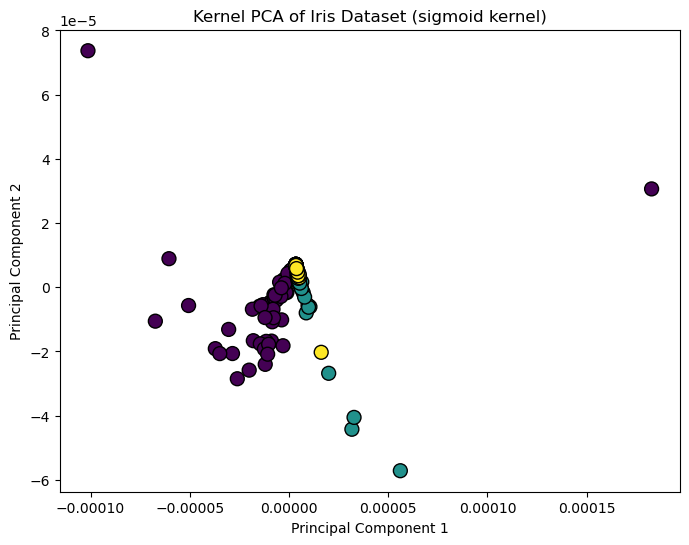
\includegraphics[width=\textwidth, height=9cm]{figures/sigmoid_kernel.png}\caption{Demonstrates the poor performance of sigmoid kernel in PCA.}\label{fig:sigmoid_kernel}
\end{figure*}

\begin{figure*}[ht]
    \centering
    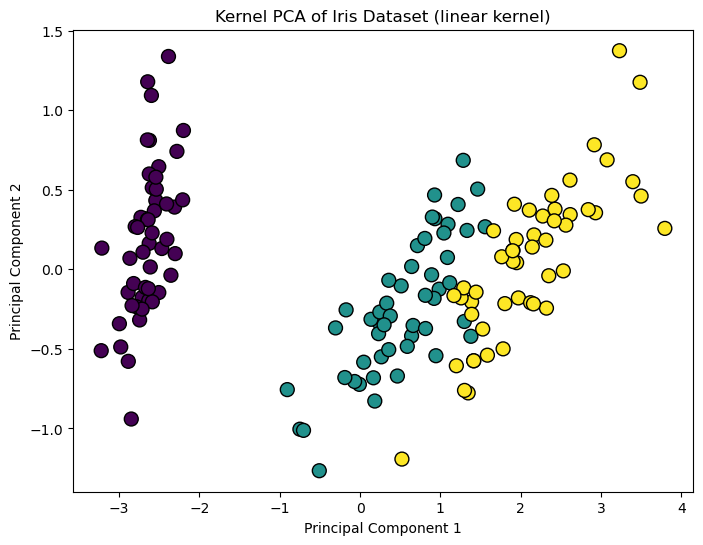
\includegraphics[width=\textwidth, height=9cm]{figures/linear_kernel_pca.png} 
    \caption{PCA using linear kernel on Iris dataset (demonstration of kernel PCA).}\label{fig:linear_kernel_pca}
\end{figure*}

figure~\ref{fig:linear_kernel_pca} shows the PCA result using linear kernel on Iris dataset. Linear kernel and RBF kernel performs well on this dataset as it is nearly linearly seperable.

\subsection{6- Build a pipeline to tune the hyperparameters of Kernel PCA and also the neural network. Which
hyperparameters can be tuned?}

Using \texttt{Pipeline} and \texttt{GridSearchCV} from \texttt{sklearn.model\_selection}, we built a pipeline to tune the hyperparameters of Kernel PCA and the MLPClassifier. The hyperparameters that can be tuned for kernel PCA are:

\begin{itemize}
    \item number of components in Kernel PCA
    \item Kernel type (linear, sigmoid, RBF)
    \item gamma value for RBF and sigmoid kernels
    \item coef0 value for sigmoid kernel
\end{itemize}

For MLPClassifier, the hyperparameters that can be tuned are:
\begin{itemize}
    \item Neural network solver (adam, sgd, lbfgs)
    \item Number of components
    \item Neural network hidden layer sizes
    \item Neural network activation function
    \item Neural network learning rate
    \item Neural network max iterations
    \item Neural network regualarization parameter (alpha)
\end{itemize}


\section{Classification Problem}



\section{Regression Problem}




\bibliographystyle{IEEEtran}
\bibliography{references}

%\textbf{Important for each reference is that it is a clickable doi that makes it easy for a reader to get hold of the reference directly (see examples in bib file).}

\end{document}


